\documentclass[10pt]{beamer}
\mode<presentation>{
   \usetheme{Warsaw}
   \usecolortheme{crane}
   \setbeamercovered{transparent}
}

\usepackage{amsfonts}
\usepackage{amsmath}
\usepackage{amssymb}
\usepackage{graphicx}

\usepackage[english]{babel}

\usepackage[utf8]{inputenc}
\usepackage{lmodern}
\usepackage[T1]{fontenc}
% Or whatever. Note that the encoding and the font should match. If T1
% does not look nice, try deleting the line with the fontenc.

\usepackage{bm}

\title[Smoothed Particle Hidrodynamics]
{Smoothed Particle Hidrodynamics for Impact Simulations}

%\subtitle
%{Presentation Subtitle} % (optional)

\author[A. González-Mancera et al.] % (optional, use only with lots of authors)
{A.~González Mancera\inst{1} \and D.~Luna\inst{1} \and C.~Alfonso\inst{1}}
% - Use the \inst{?} command only if the authors have different
%   affiliation.

\institute[Universidad de los Andes] % (optional, but mostly needed)
{
  \inst{1}%
  Department of Mechanical Engineering\\
  Universidad de los Andes
}
% - Use the \inst command only if there are several affiliations.
% - Keep it simple, no one is interested in your street address.

\date[APS - DFD 2015] % (optional)
{\today/\textit{Waiting for a conference}}

\subject{Talks}
% This is only inserted into the PDF information catalog. Can be left
% out. 



% If you have a file called "university-logo-filename.xxx", where xxx
% is a graphic format that can be processed by latex or pdflatex,
% resp., then you can add a logo as follows:

\pgfdeclareimage[height=0.75cm]{university-logo}{uniandes}
\logo{\pgfuseimage{university-logo}}

% If you wish to uncover everything in a step-wise fashion, uncomment
% the following command: 

%\beamerdefaultoverlayspecification{<+->}


\begin{document}

\begin{frame}
  \titlepage
\end{frame}

 \begin{frame}{Outline}
   \tableofcontents
%   % You might wish to add the option [pausesections]
 \end{frame}


% Since this a solution template for a generic talk, very little can
% be said about how it should be structured. However, the talk length
% of between 15min and 45min and the theme suggest that you stick to
% the following rules:  

% - Exactly two or three sections (other than the summary).
% - At *most* three subsections per section.
% - Talk about 30s to 2min per frame. So there should be between about
%   15 and 30 frames, all told.

\section{Introduction}

\subsection{Problem statement}


  % - A title should summarize the slide in an understandable fashion
  %   for anyone how does not follow everything on the slide itself.
  
%  \begin{figure}[htbp]
%   \centering
%      \includegraphics[height=2in]{motivacion.pdf}
%   \label{fig:comparacionhiper-hipo}
%  \end{figure}
%  \begin{itemize}
%   \item DPPC vesicle suspended in less dense fluid and moving due to electric fields.
%  \end{itemize}
\begin{frame}{Motivation}

\end{frame}


\subsection{Project Description}
\begin{frame}{Objectives}
\begin{Large}
\begin{center}
   Integrate bullet deformation \& target fracture in SPH simulations
\end{center}
\end{Large}
   \begin{itemize}
   \item Apply SPH Matlab routines from reference
   \item Develop new SPH formulations
   \item Implement Algorithm Modifications
   \item Evaluate Performance
   \item Manage code by version control software
   \end{itemize}
\end{frame}


\begin{frame}{General Description}
Smoothed Particle Hydrodynamics (\textit{SPH})
\begin{itemize}
\item Numerical method for approximating PDEs solutions
\item Meshless*
\item A set of \textit{particles} represent the total physical domain
\item Langrangian description*
\item Applications on Astrophysics, CFD, Solid Mechanics...
\end{itemize}
\end{frame}


\section{SPH Formulation}

\subsection{Physical Model}

\begin{frame}{Integral Representation}
A function and its spatial derivative can be represented in an integral form
$$f(x)=\int_{\Omega}{f(x')W(x-x',h)dx'}$$
$$\nabla\cdot f(x)=-\int_{\Omega}{f(x')\cdot\nabla W(x-x',h)dx'}$$
\begin{itemize}
%\item $x$ $x'$: spatial vectors
%\item $f(x)$: Function of $x$
\item $\Omega$: Defined domain for $f(x)$
\item $W$: Smoothing function (\textit{kernel*})
\item $h$: Smoothing length
\end{itemize}
\end{frame}


\begin{frame}{Smoothing Function (\textit{kernel})}
Kernel properties $W(c-x',h)$
\begin{figure}[h!]
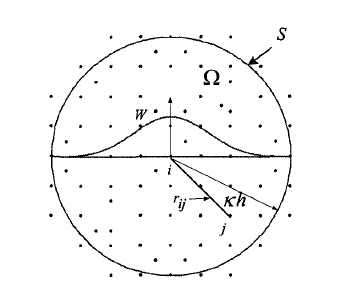
\includegraphics[scale=.5]{./images/ParticleApprox.PNG}
\end{figure}
$$\lim_{h\to0}{W(x-x',h)}=\delta(x-x')$$
$$\int_{\Omega}W(x-x',h)dx'=1$$
$$W(x-x')=0\text{, for }|x-x'|>kh$$
\end{frame}

\begin{frame}{Conservation Equations}
Continuum domain
\begin{itemize}
\item Continuity
\[\frac{D\rho}{Dt}=-\rho\frac{\partial \nu^\beta}{\partial x^\beta}\]
\item Momentum
\[\frac{D\nu^\alpha}{Dt}=\frac{1}{\rho}\frac{\partial\sigma^{\alpha\beta}}{\partial x^\beta}\]
\item Energy
\[\frac{De}{Dt}=\frac{\sigma^{\alpha\beta}}{\rho}\frac{\partial\nu^\alpha}{\partial x^\beta}\]
\end{itemize}
Stress tensor* $\sigma^{\alpha\beta}$
\end{frame}

\begin{frame}{Constitutive Model}
Stress tensor
\[\sigma^{\alpha\beta}=-P\delta^{\alpha\beta}+\tau^{\alpha\beta}\]
Jaumann
\[\dot{\tau}^{\alpha\beta}=G\left(\epsilon^{\alpha\beta}-\frac{1}{3}\delta^{\alpha\beta}\epsilon^{\gamma\gamma}\right)+\tau^{\alpha\gamma}R^{\beta\gamma} + \tau^{\alpha\beta}R^{\alpha\gamma}\]
Mie Gruniensen
\[P(e,\rho)=\left(1-\frac{1}{2}\Gamma\eta\right)P_H\rho+\Gamma\rho e\]
\begin{itemize}
\item $G$ is the shear modulus
\item $R$ si the rotation tensor
\item $P_H$ refers to Hugoniot curve
\item $\Gamma$ is the Gruneinsen Parameter
\item $\eta$ is the density change rate
\end{itemize}
\end{frame}

\begin{frame}{Material Model}
Grady \& Kipp fragmentation model
\begin{itemize}
\item Existence of incipient flaws
\item Number of flaws per unit volume $n(\epsilon)=k\epsilon^m$
\item Local stress-release due to grow of cracks\\
'Damage' $D$ $0\leq\ D \leq1$
\[\sigma_D=\sigma(1-D)\]
\end{itemize}
\end{frame}

\subsection{Particle Aproximation}
\begin{frame}{Particle Aproximation}
Contiuum $\to$ Discrete
\begin{itemize}
\item Function
\[f(x_i)=\sum_{j=1}^{N}{\frac{m_j}{\rho_j}f(x_j)W_{ij}}\]
\[W_{ij}=W(x_i-x_j,h)\]
\item Function Spatial Derivative
\[ \nabla\cdot f(x_i)=\sum_{j=1}^{N}{\frac{m_j}{\rho_j}f(x_j)\cdot\nabla_i W_{ij}}\]
\[\nabla_iW_{ij}=\frac{x_i-x_j}{r_{ij}}\frac{\partial W_{ij} }{\partial r_{ij}}=\frac{x_{ij}}{r_{ij}}\frac{\partial W_{ij}}{\partial r_{ij}}\]
\end{itemize}
\end{frame}

\begin{frame}{Conservation Equations}
Discrete Domain
\begin{itemize}
\item Conservation of mass
\[\rho_i=\sum_{j=1}^{N}{m_jW_{ij}}\]
\item Momentum
\[\frac{D\nu_i^{\alpha}}{Dt}=\sum_{j=1}^{N}{m_j\frac{\sigma_i^{\alpha\beta}+\sigma_j^{\alpha\beta}}{\rho_i\rho_j}\frac{\partial W_{ij}}{\partial x_i^\beta}}\]
\item Energy
\[\frac{De_i}{Dt}=\sum_{j=1}^{N}m_j\frac{\rho_i+\rho_j}{\rho_i\rho_j}\nu_{ij}^\beta\frac{\partial W_{ij}}{\partial x_i^\beta}+\frac{\mu_i}{2\rho_i}\epsilon_i^{\alpha\beta}\epsilon_j^{\alpha\beta}\]
\end{itemize}
\end{frame}

\begin{frame}{Material Model}
 Material model in discrete domain

\end{frame}

\section{Results}
\subsection{Simmulations}
\begin{frame}{Tensile Road}
\begin{figure}[h!]
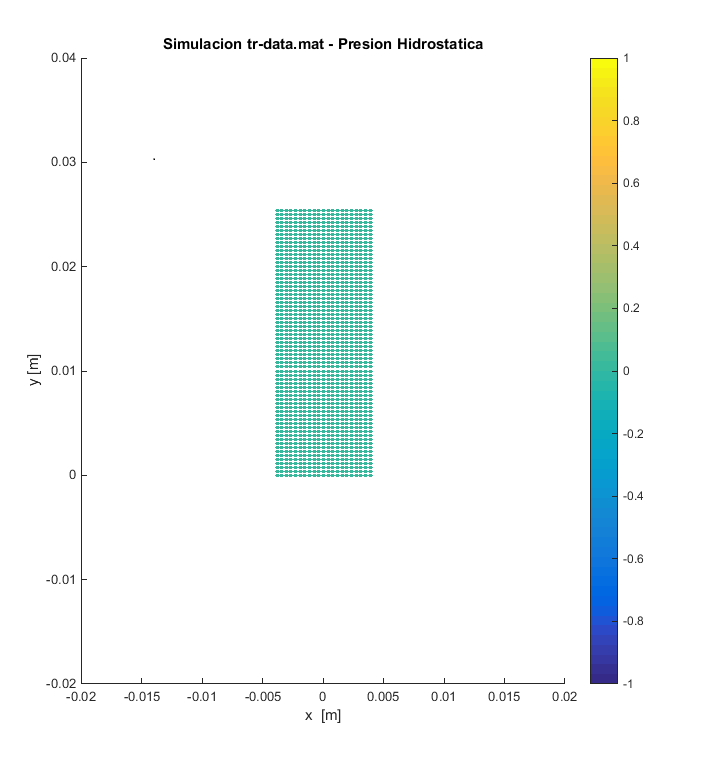
\includegraphics[scale=.25]{./images/tr_i.png}
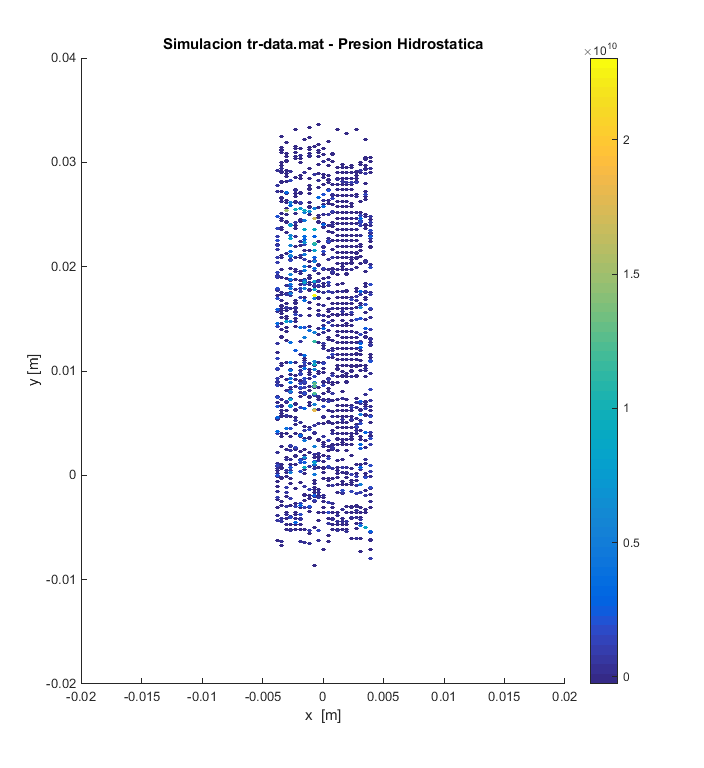
\includegraphics[scale=.25]{./images/tr_f.png}
\caption{Fracture simulation of basalt road in tension}
\end{figure}
\end{frame}

\begin{frame}{Bullet Impact}
\begin{figure}[h!]
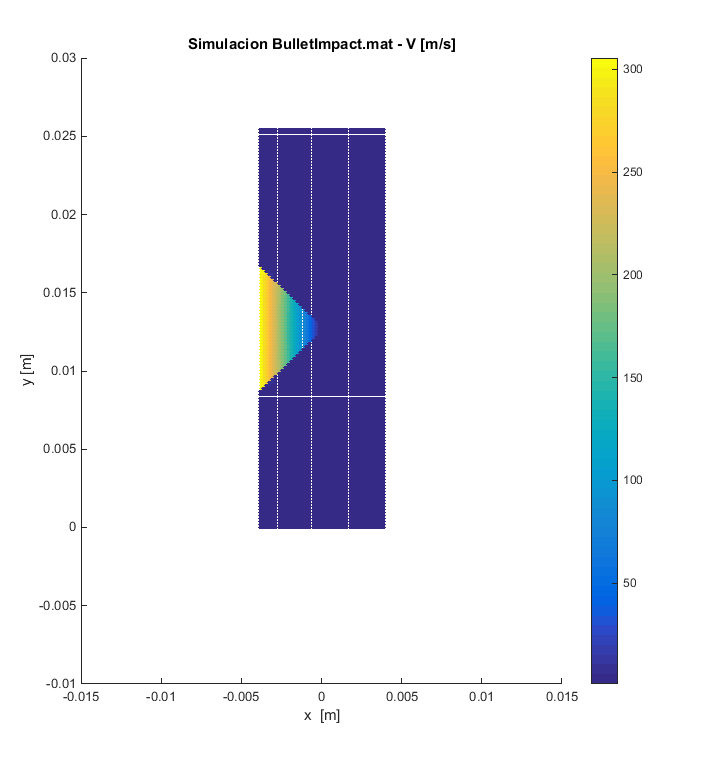
\includegraphics[scale=.25]{./images/BI_i.png}
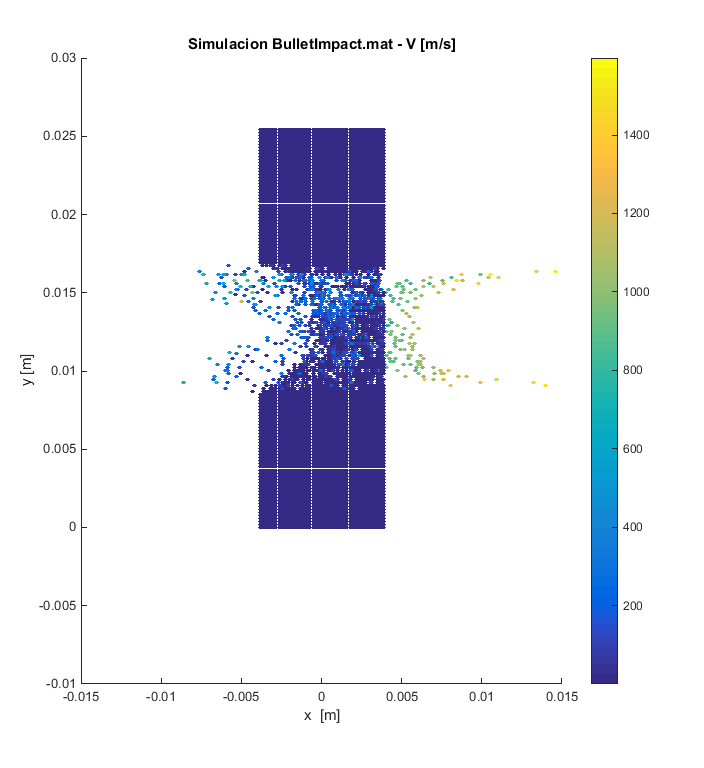
\includegraphics[scale=.25]{./images/BI_f.png}
\caption{Simulation of Basalt tarjet under initial speed dsitribution}
\end{figure}
\end{frame}

\begin{frame}{Basalt bullet impacting on basalt tarjet}
\begin{figure}[h!]
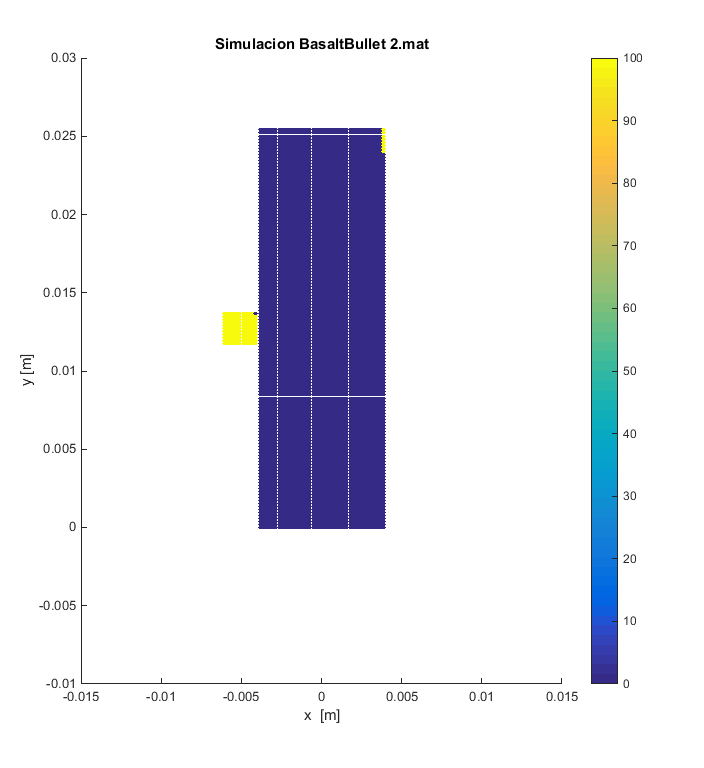
\includegraphics[scale=.25]{./images/BonB_i.png}
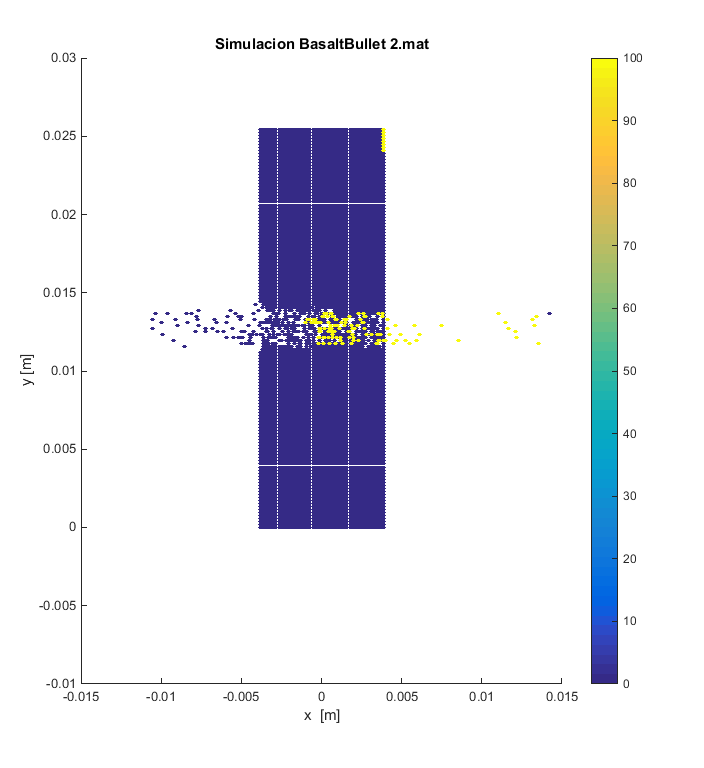
\includegraphics[scale=.25]{./images/BonB_f.png}
\caption{Simulation of Basalt bullet at initial velocity of $v_x=300 m/s$ impacting on basalt tarjet}
\end{figure}
\end{frame}

\end{document}